\documentclass[../mech.tex]{subfiles}
\graphicspath{{\subfix{../figures/}}}
\begin{document}
\chapter{Torque and Rotational Dynamics}
\section{Rotational Kinematics}
Angular displacement is the measurement of the angle, in radians, through which a point on a rigid system rotates about a specific axis.
\begin{itemize}
    \item In general, the counterclockwise motion is positive, and the clockwise motion is negative.
\end{itemize}

Angular velocity is the rate at which angular displacement position changes with respect to time.
\[ \omega = \frac{\dd \theta}{\dd t} \]

Angular acceleration is the rate at which angular velocity changes with respect to time.
\[ \alpha = \frac{\dd \omega}{\dd t} \]

Angular displacement, angular velocity, and angular acceleration around one axis are analogous to linear displacement, velocity, and acceleration in one dimension and demonstrate the same mathematical relationships.

Graphs of angular displacement, angular velocity, and angular acceleration as functions of time can be used to find the relationships between the above quantitites.

\begin{example}
    A windmill is spinning because of the nonuniform force of the wind. The windmill is originally spinning at a speed of $\omega_0$, and a crosswind slows it with an angular acceleration 
    of $-A\omega^2$. What will be the angular speed of the windmill at time $t=T$?

    From $\alpha = -A\omega^2$, we get that $\frac{1}{\omega^2}=-A$.

    Integrating this from $\omega_0$ to $\omega$ gives us $\omega = \frac{\omega_0}{\omega_0 AT + 1}$.
\end{example}

\ex Two disks, Disk 1 and Disk 2, are initially at rest and begin to rotate with a constant angular acceleration. Disk 1 has an angular acceleration $\alpha_1$ and rotates through an angle 
$\theta_1$ in a time $\Delta t$. Disk 2 has an angular acceleration $\alpha_2 = 2a_1$ and rotates through an angle $\theta_2$ in the same amount of time $\Delta t$. What is $\theta_2$ in terms of $\theta_1$?

\ex A wheel spins with an initial angular velocity of 18 rad/s in the clockwise direction and a constant angular acceleration. After 3 seconds the wheel is spinning at 6 rad/s in the counterclockwise direction. What is the magnitude and direction of the angular acceleration?

\section{Connecting Linear and Rotational Motion}
For a point at a distance $r$ from a fixed axis of motion, the linear distance $s$ traveled by the point as the system rotates through an angle $\Delta \theta$ is given by the equation 
\[ s=r\Delta \theta \]

Derived relationships of linear velocity and of the tangential component of acceleration to their respective angular quantities are given by the following equations 
\[ x=r\theta \]
\[ v = r\omega\]
\[ a=r\alpha\]
For a rigid system, all points within that system have the same angular velocity and angular acceleration.

\ex A car with tires of radius $r_0$ is moving along a straight road. Each tire's angular displacement is given by the equation $\theta = At^4+Bt$, where $t$ is time and $A$ and $B$ are constants 
with appropriate units. The tires do not slip on the road's surface. What is the car's acceleration as a function of time?

\ex \begin{center}
    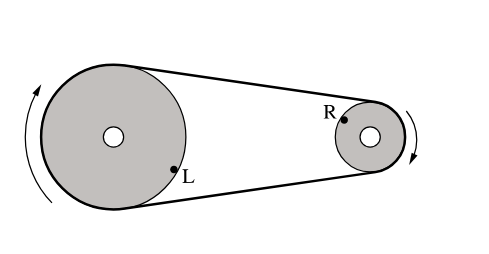
\includegraphics[width=0.5\textwidth]{5.2.PNG}
\end{center}
Two disks each rotate about axes through their centers, and are connected by a belt that does not slip as the disks rotate, as shown in the figure. The disk on the left has a larger radius than the disk on the right.
Points $L$ and $R$ are points at the edges of the disks on the left and right, respectively. Are the angular speeds and linear speeds of points $L$ and $R$ the same or different?

\section{Torque}
Torque results only from the force component perpendicular to the position to the position vector from the axis of rotation to the point of the application of the force.

The lever arm is perpendicular distance from the axis of rotation to the line of action of the exerted forces.

Torques can be described using force diagrams.
\begin{itemize}
    \item These are sometimes referred to as a rigid body diagrams.
    \item The forces are placed on the object at the point of application in relation to the axis of rotation.
\end{itemize}

The torque exerted on a rigid system about a chosen pivot point by a given force is described by 
\[ \vec{\tau}=\vec{r}\times \vec{F} \]
\[ ||\tau||=rF\sin\theta \]
The direction of the torque is determined by using the right hand curl rule.

\begin{example}
    A torque of $5.00\times 10^3$ N$\cdot$m is required to raise a drawbridge (see the following figure). What is the tension necessary to produce this toruqe? Would it be easier to raise the drawbridge if the angle $\theta$ were larger or smaller?

    \begin{center}
        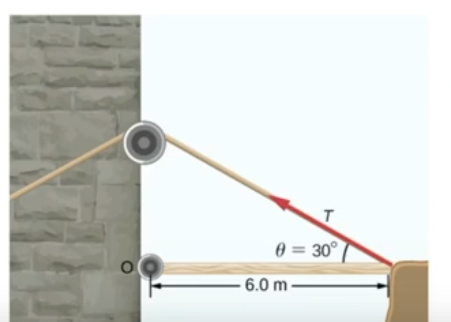
\includegraphics[width=0.5\textwidth]{5.3.1.PNG}
    \end{center}

    Just plug into the formula. $\tau = rF\sin\theta \implies T=\frac{\tau}{r\sin\theta}=1700$N.

    If you increase $\theta$, the tension would be smaller.
\end{example}

\ex \begin{center}
    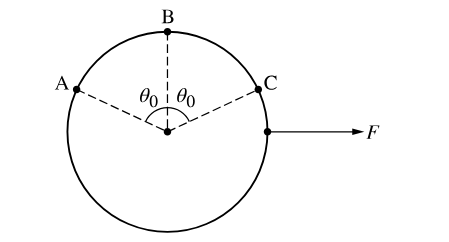
\includegraphics[width=0.5\textwidth]{5.3.2.PNG}
\end{center}
A force $F$, directed to the right, is exerted on a disk, as shown in the figure. The disk may pivot in the plane of the page about any one of the three labeled points, and the force results in lever arms of length $L_A$, $L_B$, and $L_C$ for pivots at points $A$, $B$, and $C$, respectively. 
Rank $L_A,L_B$, and $L_C$.

\ex \begin{center}
    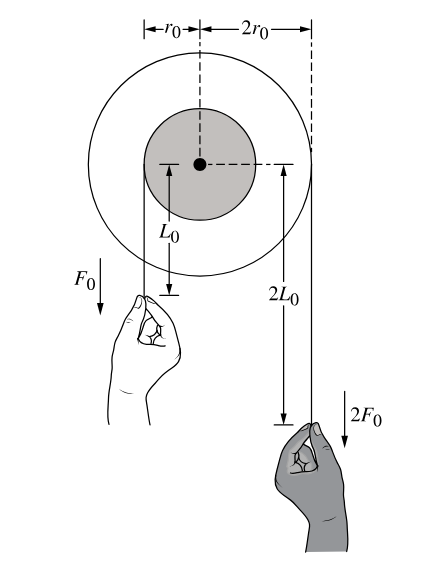
\includegraphics[width=0.5\textwidth]{5.3.3.PNG}
\end{center}
Two pulley wheels are rigidly connected so that they can rotate together around a common center, as shown in the figure. The wheels have radii $r_0$ and $2r_0$, and strings wrapped around each wheel are pulled by two students.
One student pulls downward on the smaller wheel's string with a force of magnitude $F_0$ exerted a vetical distance $L_0$ below the wheels' center. The other student pulls downward on the larger wheel's string with a force of magnitude 
$2F_0$ exerted a distance $2L_0$ below the wheels' center. The students make the correct claim that the force $2F_0$ results in a greater torque with respect to the wheels' center. Provide the evidence needed to justify this claim.
\section{Rotational Inertia}
Rotational inertia measures a rigid system's resistance to changes in rotation and is related to the mass of the system and the distribution of the mass relative to the axis of rotation.

The rotational inertia of an object rotating a perpendicular distance $r$ from an axis is described by the equation 
\[ I=mr^2 \]

The total rotational inertia of a collection of objects about an axis is the sum of the rotational inertias of each about that that axis.
\[ I= \sum m_ir_i^2 \]

For a solid that can be considered as a collection of differential masses, $\dd m$, the solid's rotational inertia can be calculated using the equation 
\[ I = \int r^2 \dd m\] 

A rigid system's rotational inertia in a given plane is at minimum when the rotational axis passes through the system's center of mass.

The parallel axis theorem uses the following equation to relate the rotational inertia of a rigid system about any axis that is parallel to an axis through its center of mass.
\[ I'=I_{cm}+md^2 \]

\begin{example}
    A triangular rod of length $L$ and mass $M$ has a nonuniform linear mass density given by the equation $\lambda = \gamma x^2$, where $\gamma = \frac{3M}{L^3}$ and $x$ is the distance from point $P$ at the left end of the rod.
    Using integral calculus, show that the rotational inertia $I$ of the rod about an axis perpendicular to the page and through point $P$ is $\frac{3}{5}ML^2$.
    \begin{center}
        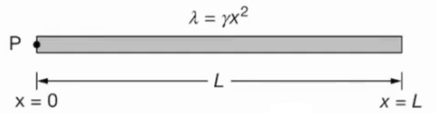
\includegraphics[width=0.5\textwidth]{5.4.PNG}
    \end{center}

    First integrate $\int_0^{L}x^2 \dd m$. We can substitute $\dd m = \gamma x^2 \dd x$, and simplifying, we get $I=\gamma \int_0^{L}x^4 \dd x$.

    Integrating this will give you $I=\frac{3}{5}ML^2$
\end{example}

\ex \begin{center}
    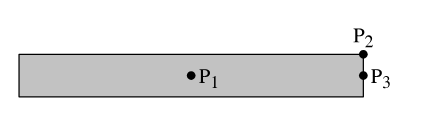
\includegraphics[width=0.5\textwidth]{5.4.1.PNG}
\end{center}
The figure shows a narrow, uniform rectangular plate. The place can rotate about any of three axes that are each perpendicular to the plane of the figure and pass through one of the points 
$P_1$, $P_2$, or $P_3$. Correctly compare the rotational inertias $I_1, I_2$, and $I_3$ of the plate about points $P_1, P_2$, and $P_3$ respectively.

\ex \begin{center}
    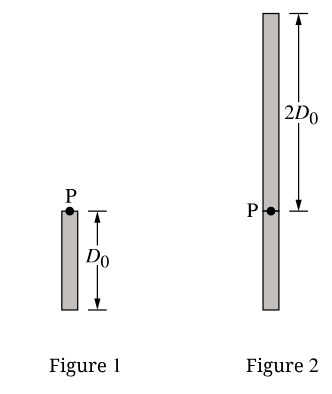
\includegraphics[width=0.5\textwidth]{4.4.2.PNG}
\end{center}
Figure 1 shows a uniform rod of mass $M_0$ and length $D_0$. Its rotational inertia when rotated about its end at point $P$ is given by $I_0=\frac{1}{3}M_0D_0^2$. A second uniform rod with twice the length 
and the same width is made of the same material, and the two rods are connected at their ends at point $P$, as shown in Figure 2. What is the rotational inertia about Point $P$ for the two-rod system in Figure 2?

\section{Newton's First and Second Law in Rotational Form}
A system may exhibit rotational equilibrium (constant angular velocity) without being in translational equilibrium, and vice versa.
\begin{itemize}
    \item FBD and force diagrams describe the nature of the forces and torques exerted on an object or rigid system.
    \item Rotational equilibrium is a configuration of torques such that the net torque exerted on the system is zero.
    \item The rotational analog of Newton's 1st law is that a system will have a constant angular velocity only if the net torque exerted on the system is zero.
\end{itemize}

A rotational collolary to Newton's 2nd law states that if the torques exerted on a rigid system are not balanced, the system's angular velocity must be changing.

Angular velocity changes when the net torque exerted on the object or system is not equal to zero.

The rate at which angular velocity of a rigid system changes is directly proportional to the net torque exerted on the rigid system as in the same direction.
\[ \sum \tau = I\alpha \]
To fully a describe a rotating rigid system, linear and rotational analyses may need to be performed independently.
\begin{example}
    A solid disk of unknown mass and known radius $R$ is used as a pulley in a lab experiment, as shown. A small block of mass $m$ is attached to a string, the other end of which is attached to the pulley and wrapped around it several times.
    The block of mass $m$ is released from rest and takes a time $t$ to fall the distance $D$ to the floor. Calculate the linear acceleration $a$ of the falling block in terms of the given quantitites.
    \begin{center}
        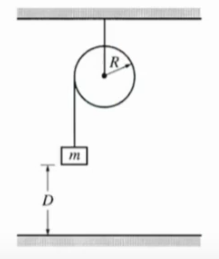
\includegraphics[width=0.5\textwidth]{5.5.PNG}
    \end{center}

    We first must find $T$, the tension.

    To find this, we can determine that $T=\frac{1}{2}ma$, from plugging in known quantities and the fact that $I=\frac{1}{2}mr^2$.

    Now the sum of the forces is $\sum F = ma$, so $T=mg-ma$.

    Solving for $a$ after plugging in everything should give $\frac{2}{3}g$.
\end{example}

\ex \begin{center}
    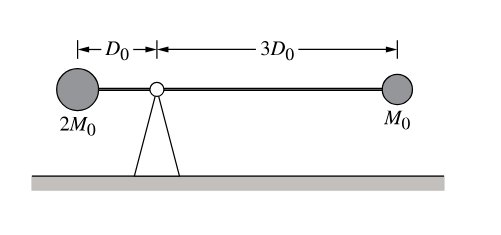
\includegraphics[width=0.5\textwidth]{5.5.1.PNG}
\end{center}
A thin rod of negligible mass has spheres of different masses attached to its ends, as shown in the figure. The rod is free to rotate about an axis perpendicular to the plane of the figure and located at a triangular fulcrum that supports the rod.
If the rod is held in place horizontally and then released from rest, what is the magnitude of the angular acceleration of the rod-spheres system immediately after the rod is released?

\ex \begin{center}
    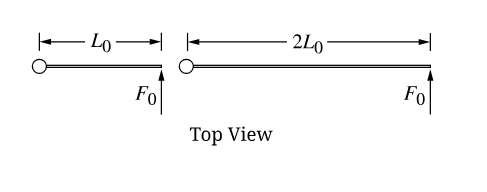
\includegraphics[width=0.5\textwidth]{5.5.2.PNG}
\end{center}
A uniform rod of length $L_0$ is free to rotate about an axis through its left end and perpendicular to the horizontal plane of the figure shown. When a force with magnitude $F_0$ is exerted perpendicular to the rod at the right end, 
the angular acceleration of the rod is $\alpha_1$. The same force is then exerted on the right end of a second uniform rod with the same linear mass density and twice the length as the original rod, as shown on the right side of the figure.
The rod of length $2L_0$ has an angular acceleration of $\alpha_2$. What is the ratio $\alpha_2:\alpha_1$?

\end{document}